\section{RLVR at 0.6B: A Pre-Registered Null}\label{sec:rlvr}

The final lifecycle stage asks whether reinforcement learning from verifiable rewards (RLVR)
adds reasoning capability on top of the SFT checkpoint at this scale. The recent literature
motivates skepticism rather than optimism. \citet{yue2025does} argue that RLVR sharpens the
distribution the base model already supports---raising pass@1 while narrowing rather than
expanding pass@$k$ coverage---and \citet{shao2025spurious} show that Qwen-lineage models
improve under spurious and even random rewards, so an RLVR gain claimed on this lineage is
uninterpretable without a random-reward control. The stage plan (researched 2026-07-01, one
day before the 2026-07-02 launch) therefore pre-registered both the prediction and the
decision rule: on this FineWeb-Edu$\to$SFT base, which the plan characterizes as roughly
$10\times$ undertrained relative to compute-optimal token budgets \citep{hoffmann2022training},
RLVR is expected to sharpen rather than expand, ``the most likely true outcome is a
null-or-tiny attributable Dr.GRPO gain that the control battery should correctly refuse to
call a win,'' and a win may be declared only if GRPO beats \emph{both} the SFT floor and a
mandatory random-reward gate arm, with ``beats'' fixed in advance as non-overlapping Wilson
95\% confidence intervals.

\begin{figure}[t]
\centering
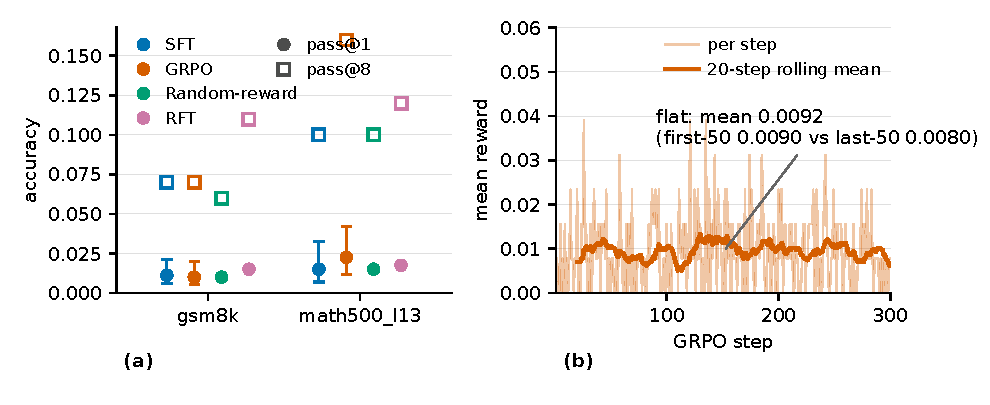
\includegraphics[width=\linewidth]{figures/fig_rlvr.pdf}
\caption{RLVR at 596M: pass@1 (Wilson 95\% CIs) and pass@8 \citep{chen2021evaluating} for the
SFT floor, Dr.GRPO, the random-reward gate arm, and the iso-generation-compute RFT control on
GSM8K (100 items) and MATH-500 levels 1--3 (50 items), 8 samples per item at $T{=}0.8$, band
seed 20260701, $n{=}1$ training seed, verifier pinned as \texttt{math-acc-v1}. GRPO trained
300 steps $\times$ 16 prompts $\times$ $G{=}8$ rollouts; its training reward stayed flat at
$\approx$0.9\% verifier-correct with no trend. All arm CIs overlap and both pre-registered
gates fail. Source files: \texttt{phase1\_passk.json}, \texttt{passk\_grpo.json},
\texttt{passk\_random.json}, \texttt{passk\_rft.json}, \texttt{health\_grpo\_seed0.jsonl}.}
\label{fig:rlvr}
\end{figure}

% tab_rlvr.tex -- RLVR Phase-2 paired eval: SFT floor / GRPO / random-reward gate / RFT control,
% on gsm8k (100 items) and math500_l13 (50 items), 8 samples each, plus the two pre-registered gates.
% Sources in Qwen3-0.6B/experiments/:
%   2026-07-01_qwen3-0.6b_rlvr-phase1-passk/phase1_passk.json (SFT + base cells, same band)
%   2026-07-02_qwen3-0.6b_grpo-phase2/passk_grpo.json, passk_random.json, passk_rft.json, verdict.json (gates)
\begin{table}[t]
\centering
\caption{RLVR at 596M: paired pass@$k$ of the SFT floor, Dr.GRPO, the random-reward (Spurious-Rewards) gate arm, and the iso-generation-compute RFT control, all decoded on the same band (100 GSM8K $+$ 50 MATH-500 level-1--3 items, 8 samples per item, $T{=}0.8$, max 256 new tokens, band seed 20260701; answer verifier pinned as \texttt{math-acc-v1}; both eval sets 0-flagged in a 13-gram decontamination check against the 35{,}924 SFT problems).
GRPO trained 300 steps $\times$ 16 prompts $\times$ $G{=}8$ rollouts; its training reward stayed flat at $\approx$0.9\% verifier-correct with no trend.
The RFT control collected 352 verifier-correct completions ($\approx$0.9\% of 38{,}400 rollouts) --- not 0, as an earlier draft misread from a smoke-test log line.
pass@1 carries a Wilson 95\% CI; pass@8 is the Chen et al.\ (2021) unbiased estimator; a gate ``passes'' only on non-overlapping Wilson CIs.
Both pre-registered gates FAIL on both sets, confirming the pre-registered null; RFT is nominally best on GSM8K (pass@8 11\% vs.\ 7\%) and GRPO on MATH-500 (16\% vs.\ 10\%), but all CIs overlap (n.s.), and GRPO's MATH-500 pass@1 merely ties the pretrain base (2.25\%).
$n{=}1$ seed, so the verdict is capped at \emph{directional}; phase 3 not launched.
Source files: \texttt{phase1\_passk.json} (SFT, base), \texttt{passk\_grpo.json}, \texttt{passk\_random.json}, \texttt{passk\_rft.json}, \texttt{verdict.json}.}
\label{tab:rlvr}
\footnotesize
\begin{tabular}{lcccc}
\toprule
 & \multicolumn{2}{c}{GSM8K (100 items)} & \multicolumn{2}{c}{MATH-500 L1--3 (50 items)} \\
\cmidrule(lr){2-3} \cmidrule(lr){4-5}
Arm & pass@1 \% (Wilson 95\%) & pass@8 \% & pass@1 \% (Wilson 95\%) & pass@8 \% \\
\midrule
SFT (floor)          & 1.12 $[0.59,\,2.12]$ & 7  & 1.50 $[0.69,\,3.23]$ & 10 \\
GRPO                 & 1.00 $[0.51,\,1.96]$ & 7  & 2.25 $[1.19,\,4.22]$ & 16 \\
Random reward (gate) & 1.00 $[0.51,\,1.96]$ & 6  & 1.50 $[0.69,\,3.23]$ & 10 \\
RFT (iso-gen.\ control) & 1.50 $[0.86,\,2.60]$ & 11 & 1.75 $[0.85,\,3.57]$ & 12 \\
\addlinespace
Base (reference, Phase 1) & 0.62 $[0.27,\,1.45]$ & 5 & 2.25 $[1.19,\,4.22]$ & 14 \\
\midrule
\multicolumn{5}{l}{\emph{Pre-registered gates (non-overlapping Wilson CIs required; outcome identical on both sets)}} \\
GRPO beats SFT floor    & \multicolumn{4}{c}{FAIL (\texttt{grpo\_beats\_sft\_floor} $=$ false)} \\
GRPO beats random gate  & \multicolumn{4}{c}{FAIL (\texttt{grpo\_beats\_random\_gate} $=$ false)} \\
\bottomrule
\end{tabular}
\end{table}


All arms are decoded on one fixed band: 100 GSM8K test items \citep{cobbe2021training} and 50
MATH-500 level-1--3 items \citep{hendrycks2021measuring}, 8 samples per item at temperature
0.8 with at most 256 new tokens, band seed 20260701. pass@1 carries a Wilson 95\% CI; pass@8
is the unbiased estimator of \citet{chen2021evaluating}; answers are scored by a pinned,
version-stamped verifier (math-acc-v1). Contamination was checked before any number was read:
a 13-gram index against the 35{,}924 SFT problems flags zero items in either eval set, and 14
eval-overlapping prompts were dropped from the GRPO training-prompt pool
(Table~\ref{tab:rlvr}).

A cheap Phase-1 gate preceded any RL spend. On this band (math-acc-v1) the SFT checkpoint
scores 1.1\% pass@1 on GSM8K (Wilson 95\% CI $[0.6, 2.1]$) and 7\% pass@8, and 1.5\%/10\% on
MATH-500 L1--3; the pretraining base scores 0.6\%/5\% and 2.25\%/14\% respectively
(Table~\ref{tab:rlvr}). The pre-registered GO rule was absolute solvability---proceed if and
only if the SFT arm solves at least 3 items across the band---and it fired with 12 solved
items. What the gate did \emph{not} establish should be stated plainly: GO fired on absolute
solvability, not on SFT beating the base. The SFT and base intervals overlap on every cell,
and the base beats SFT on MATH-500 pass@8 (14\% vs.\ 10\%)---an early warning that arm
separations near this accuracy floor sit inside the noise.

Phase 2 trained Dr.GRPO \citep{liu2025understanding} from the SFT checkpoint for 300 steps of
16 prompts $\times$ $G{=}8$ rollouts (38{,}400 rollouts total, at a measured $\approx$362~s
per step; roughly 88 hours estimated for the three arms): clip ratio 0.2, k3 KL penalty to the
frozen SFT reference with $\beta = 3\times10^{-3}$ (a coefficient flagged as inferred, not
paper-pinned), learning rate $10^{-6}$, and DAPO-style filtering of zero-variance rollout
groups \citep{yu2025dapo}, which retained 13.49 of 16 groups per step on average
(Table~\ref{tab:hparams})---the update was not gradient-starved. The training signal never
moved: the per-step verifier-correct rate (the fraction of the 128 rollouts per step scoring
exactly 1.0, not the shaped reward) is flat at $\approx$0.9\% (mean 0.0092; first-50-step
mean 0.009 vs.\ last-50 0.008; OLS slope $+5.8\times10^{-7}$ per step), and the per-token KL
to the reference stays near $1.7\times10^{-4}$ throughout, i.e., the policy barely moved
(Figure~\ref{fig:rlvr}). Two controls ran under the same recipe. The random-reward gate arm
\citep{shao2025spurious} replaced the verifier with a content-blind Bernoulli(0.5) draw and
trained at reward $\approx$0.5, confirming that the sampling, advantage, and update pipeline
all function. The RFT control spent iso-generation compute: it drew the same 38{,}400
rollouts, collected the 352 verifier-correct completions ($\approx$0.9\% of rollouts,
consistent with the GRPO reward floor), and ran one masked SFT pass over 200 of them.

Table~\ref{tab:rlvr} reports the final paired evaluation of all four arms on the same band
(math-acc-v1). On GSM8K, GRPO scores 1.0\% pass@1 / 7\% pass@8 against the SFT floor's
1.12\%/7\%, the random-reward arm's 1.0\%/6\%, and RFT's 1.5\%/11\%. On MATH-500 L1--3, GRPO's
nominal bump to 2.25\%/16\% over SFT's 1.5\%/10\% resembles the expected sharpening story
until it is compared with the pretraining base: GRPO's MATH-500 pass@1 of 2.25\% exactly
equals the base checkpoint's Phase-1 value on the same band, so the ``gain'' does not clear
the model the SFT stage started from. Both pre-registered gates fail on both eval sets: the
GRPO intervals overlap the SFT floor's and the random-reward gate's everywhere
(\texttt{grpo\_beats\_sft\_floor} and \texttt{grpo\_beats\_random\_gate} both evaluate to
false). The one nominally interesting cell---RFT's 11\% pass@8 on GSM8K against the floor's
7\%---is not significant (overlapping CIs) and, at one training seed, is at most a hypothesis
for future work.

The recorded verdict is \emph{directional}, capped by design rather than by accident: the
per-stage evaluation-completeness gate requires at least three paired seeds for any
non-directional RLVR call, and this cohort deliberately ran one seed with
proceed-to-phase-3 set to false---buying two further seeds would only have tightened a
confidence interval around zero. The pre-registered null is confirmed: at 0.6B, on this
undertrained base, the measurable reasoning gain arrived with SFT, not with RL, consistent
with the sharpen-not-expand account of \citet{yue2025does} and the Qwen-lineage
spurious-reward findings of \citet{shao2025spurious}. The claim is deliberately bounded. It
says nothing about RLVR at larger scales, on stronger bases, or with longer training; it says
that at this scale, under the controls the literature itself demands, an honest evaluation
battery refuses to call RLVR a win---and that a control battery designed before launch is
what makes such a refusal cheap.
